\section{Thin\-Lens Class Reference}
\label{classThinLens}\index{ThinLens@{ThinLens}}
Thin lens elements (linear and nonlinear). 


{\tt \#include $<$Sector\-Map.h$>$}

Inheritance diagram for Thin\-Lens::\begin{figure}[H]
\begin{center}
\leavevmode
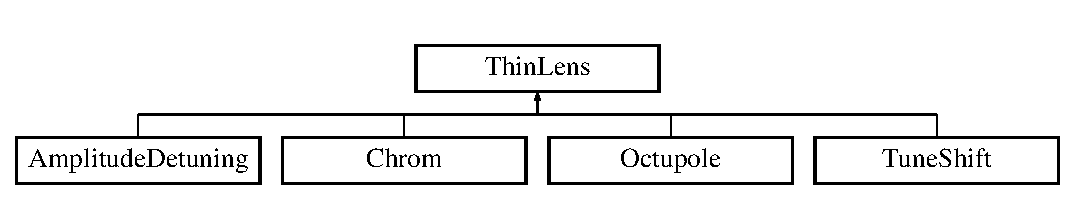
\includegraphics[height=2cm]{classThinLens}
\end{center}
\end{figure}
\subsection*{Public Member Functions}
\begin{CompactItemize}
\item 
virtual void {\bf kick} (vektor \&R1, vektor \&R0, double ds)=0\label{classThinLens_a0}

\end{CompactItemize}


\subsection{Detailed Description}
Thin lens elements (linear and nonlinear).



Definition at line 93 of file Sector\-Map.h.

The documentation for this class was generated from the following file:\begin{CompactItemize}
\item 
Sector\-Map.h\end{CompactItemize}
